% Preamble
\documentclass[xcolor=dvipsnames]{beamer}
\usetheme{madrid}

% Packages
\usepackage[english,ngerman]{babel}
\usepackage[utf8]{inputenc}
\usepackage{amsmath}
\usepackage{graphicx}
\usepackage{amssymb}

\definecolor{hBlue}{RGB}{55,118,165}
\usecolortheme[named=hBlue]{structure}

\titlegraphic{
\includegraphics[width=4cm]{../images/logo.png}}
\title{Gesundheit \& Ernährung}
\subtitle{Vitamin D}
\author{Adrian Helberg}
\date{05.05.2021}

% Document
\begin{document}

    \maketitle

    \frame{\frametitle{Agenda}\tableofcontents}

    \section{Theorie}
    {
    \setbeamercolor{normal text}{fg=hBlue}\usebeamercolor*{normal text}
    \begin{frame}
        \begin{center}
            \Huge Theorie
        \end{center}
    \end{frame}
    }

    \subsection{Aktueller Stand}
    \begin{frame}[allowframebreaks]
        \frametitle{Aktueller Stand}

        \begin{figure}
            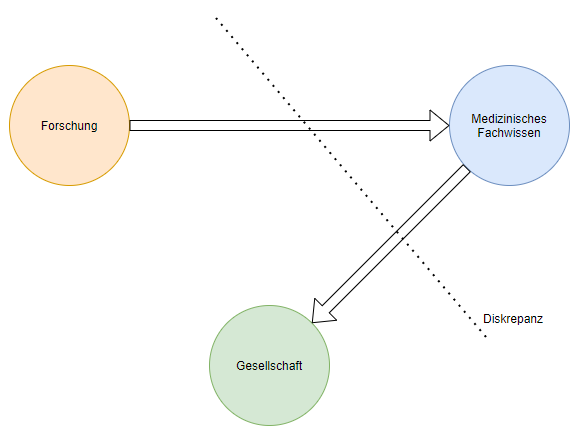
\includegraphics[width=6cm]{../images/wissensgesellschaft_3.png}
            \caption{Wissensgesellschaft}
        \end{figure}

        \framebreak

        \begin{figure}
            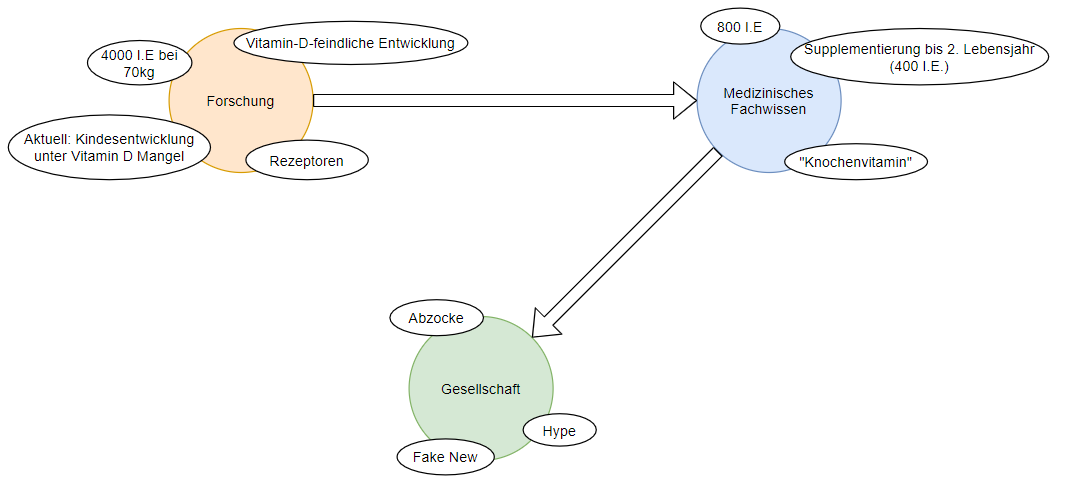
\includegraphics[width=10cm]{../images/wissensgesellschaft_vitamin_d.png}
            \caption{Wissensgesellschaft}
        \end{figure}

        \framebreak

        \begin{figure}
            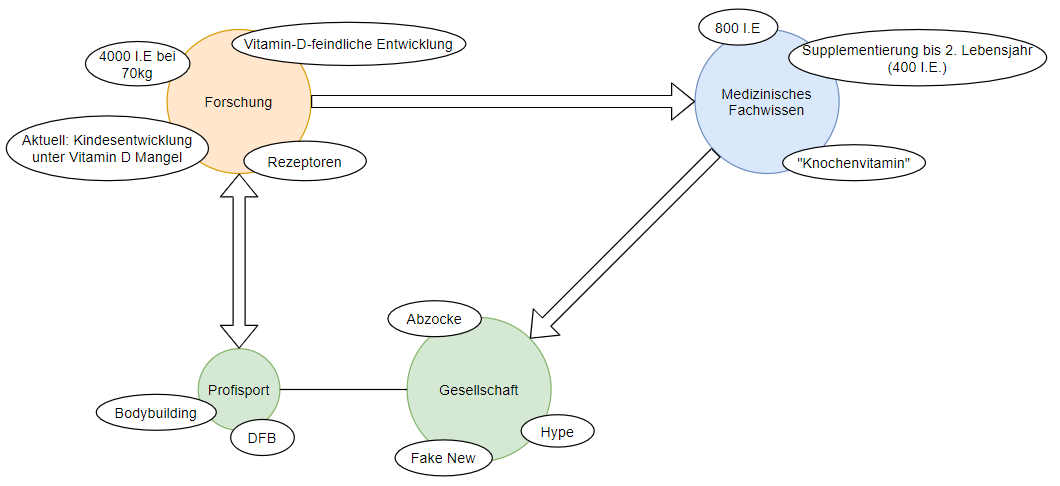
\includegraphics[width=10cm]{../images/wissensgesellschaft_vitamin_d_sport.png}
            \caption{Wissensgesellschaft}
        \end{figure}


    \end{frame}

    \subsection{Synthese}
    \begin{frame}[allowframebreaks]
        \frametitle{Vitamin D Synthese}

        \begin{figure}
            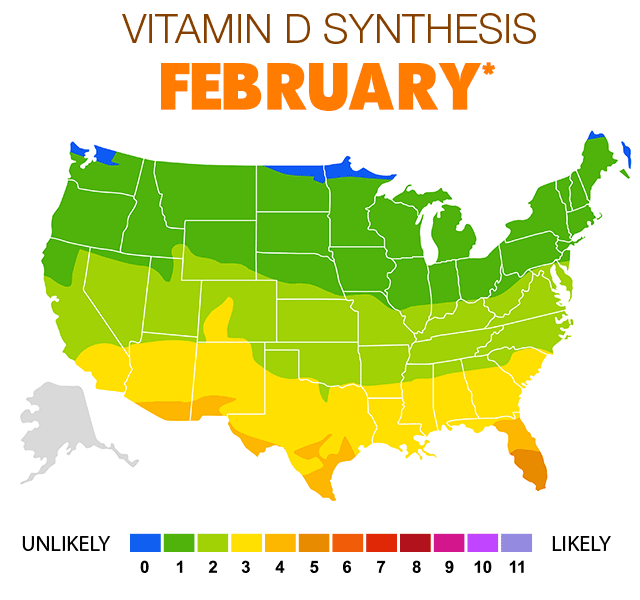
\includegraphics[width=6cm]{../images/vitamin_d_map.png}
            \caption{Vitamin-D-Synthese USA}
        \end{figure}

        \framebreak

        \begin{figure}
            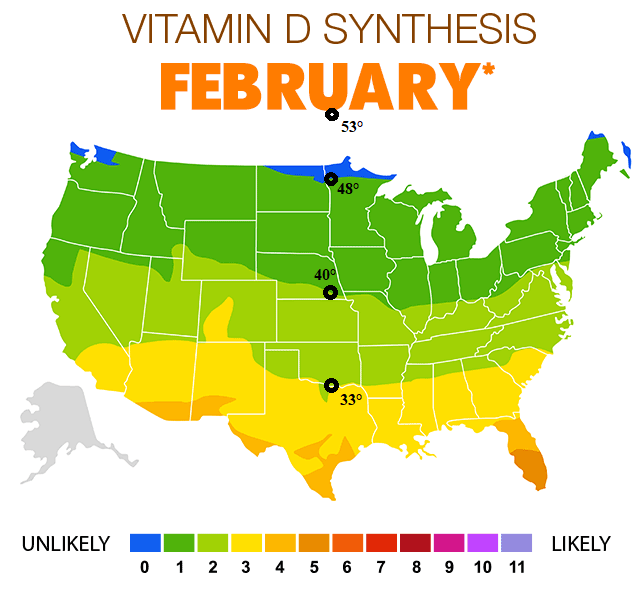
\includegraphics[width=6cm]{../images/vitamin_d_map_2.png}
            \caption{Vitamin-D-Synthese USA}
        \end{figure}

        \framebreak

        \begin{figure}
            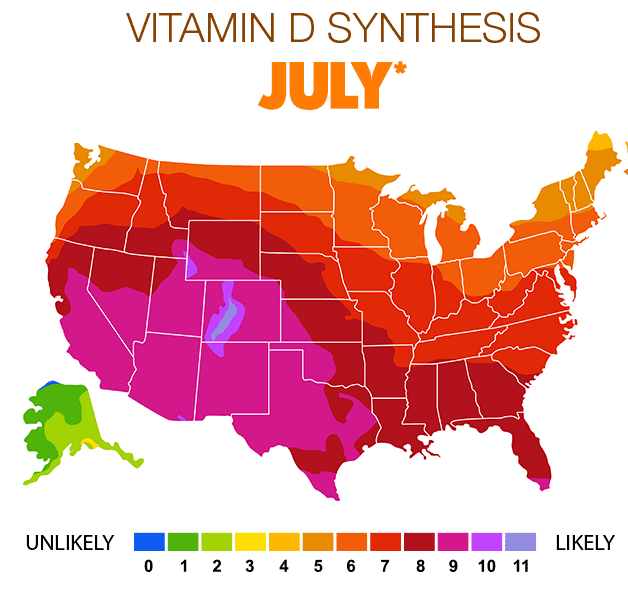
\includegraphics[width=6cm]{../images/vitamin_d_map_3.png}
            \caption{Vitamin-D-Synthese USA}
        \end{figure}

        \framebreak

        \begin{figure}
            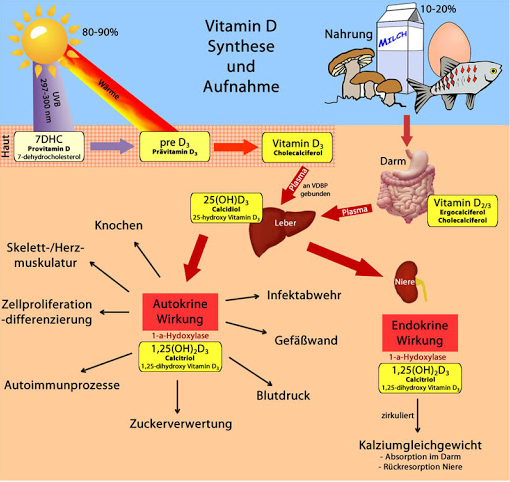
\includegraphics[width=7cm]{../images/vitamin_d_synthese.png}
            \caption{Vitamin D Aufnahme \& Synthese}
        \end{figure}
    \end{frame}

    \subsection{Dosierung}
    \begin{frame}
        \frametitle{Dosierung}
        \begin{block}{Dosierempfehlung}
            \begin{itemize}
                \setlength\itemsep{1em}
                \item Allgemeine, internationale Empfehlung: 4.000 IE / Tag
                \item 1000 IE Vitamin D / Tag fürhren zu einer Erhöhung des Blutspiegels um 10 ng/ml bei 70kg Körpergewicht
                \item Überdosierung kaum möglich
                \begin{itemize}
                    \item Sehr hohe Dosen über einen langen Zeitraum
                \end{itemize}
                \item Bei Verdacht / für Skeptiker:
                \begin{itemize}
                    \item Calciumspiegel messen lassen
                    \item Keine Überdosierung ohne Erhöhung des Calciumspiegels
                    \item Calcium sorgt dann für die Symptome
                \end{itemize}
            \end{itemize}
        \end{block}
    \end{frame}

    \subsection{Gesundheitliche Aspekte}
    \begin{frame}[allowframebreaks]
        \frametitle{Gesundheitliche Aspekte}
        \begin{center}
            Kohlenhydratisierung ~~~~~~~~~~~~~~~~~~~~~~~~~~~~~~~~~~~~~~~~~~~~~~~~~~~~~~~~~~~~\\
            $\downarrow$ ~~~~~~~~~~~~~~~~~~~~~~~~~~~~~~~~~~~~~~\\
            Insulinresistenz ~~~~~~ Fettmangel ~~~~~~~~ Vitamin D Mangel\\
            $\downarrow$ ~~~~~~~~~~~~~~~~~~ $\downarrow$ ~~~~~~~~~~~~ $\downarrow$\\
            Weniger Nahrung für die Zellen\\
            $\downarrow$\\
            Krankheiten
        \end{center}

        \framebreak

        \begin{block}{Vitamin D Abhängigkeiten, Gehirnzellen}
            \begin{itemize}
                \setlength\itemsep{1em}
                \item Multiple Sklerose
                \item Shizophrenie
                \item Depression
                \item Parkinson
                \item Demenz (Diabetes Typ 3)
                \item \ldots
            \end{itemize}
        \end{block}

        \framebreak

        \begin{block}{Vitamin D Abhängigkeiten, Bewegungsapperat}
            \begin{itemize}
                \setlength\itemsep{1em}
                \item Vitamin D beeinflusst
                \begin{itemize}
                    \item Muskelkraft
                    \item Muskelaufbau
                    \item Gleichgewicht
                    \item Muskelfunktion
                    \item \ldots
                \end{itemize}
                \item[$\rightarrow$] Vermindertes Sturzrisiko
                \item Vitamin D erhöht die Knochendichte
                \item[$\rightarrow$] Vermindertes Frakturrisiko
            \end{itemize}
        \end{block}

        \framebreak

        \begin{block}{Vitamin D Abhängigkeiten, Herz(muskel)zellen}
            \begin{itemize}
                \setlength\itemsep{1em}
                \item Herzinfarkt
                \item Herzschwäche
                \item Endokarditis (Herzklappenentzündung)
                \item \ldots
            \end{itemize}
        \end{block}

        \framebreak

        \begin{block}{Vitamin D Abhängigkeiten, Immunsystem}
            \begin{itemize}
                \setlength\itemsep{1em}
                \item Vitamin D betreibt Zellreperatur $\rightarrow$ Senkung des Krebsrisikos
                \item Gen-Schäden hat es schon immer gegeben: Sonne, kosmische Strahlung
                \item Tumorwachstum kann durch rechtzeitige Supplementierung gestoppt werden
                \item Vitamin D ist wesentlicher Bestandteil der Immunabwehr $\rightarrow$ Infektdauer sinkt
                \item Autoimmunerkrankungen
                \item \ldots
            \end{itemize}
        \end{block}

        \framebreak

        \begin{block}{Vitamin D Abhängigkeiten, Mortalität}
            \begin{figure}
                \includegraphics[width=4.4cm]{../images/vitamin_d_mortalität.png}
                \caption{Gesamtsterblichkeit und Vitamin $$}
            \end{figure}
        \end{block}
    \end{frame}

    \section{Praxis}
    {
        \setbeamercolor{normal text}{fg=hBlue}\usebeamercolor*{normal text}
        \begin{frame}
            \begin{center}
                \Huge Praxis
            \end{center}
        \end{frame}
    }

    \subsection{Tipps \& Tricks}
    \begin{frame}
        \frametitle{Nützliche Tipps \& Tricks}
        \begin{itemize}
            \item der "`Schattentrick"'
            \item Supplementierung mit 4.000 IE / Tag
            \item Halbwertszeit von 19 Tagen, aber lieber 1x pro Tag, als 1x die Woche
            \item die Deutsche Gesellschaft für Ernährung (DGE) ist eine schlechte Quelle in Gesundheitsfragen
            \item Keine klare Symptomatik für Unterversorgung $\rightarrow$ das schwächste Glied des Körpers erkrankt
        \end{itemize}
    \end{frame}

    \section{Fragerunde}
    {
        \setbeamercolor{normal text}{fg=hBlue}\usebeamercolor*{normal text}
        \begin{frame}
            \begin{center}
                \Huge Fragerunde
            \end{center}
        \end{frame}
    }

\end{document}
